\chapter{环境配置}

\section{Linux环境配置}
Windows和MacOS是当前最流行的两个操作系统,其中,MacOS是类Unix系统,与Linux共享编程语言,因此你可以在Terminal中直接使用Linux相关指令。如果你是Windows系统,你需要安装Linux子系统或虚拟机。

\subsection{Windows Subsystem for Linux, WSL}
WSL是Windows Subsystem for Linux的缩写,是一个在Windows 10上能够运行原生Linux二进制可执行文件(ELF格式)的兼容层。它是由微软与Canonical公司合作开发,其目标是使纯正的Ubuntu、Debian等映像能下载和解压到用户的本地计算机,并且映像内的工具和实用工具能在此子系统上原生运行。

WSL提供了一个完整的Linux内核,但它不是一个虚拟机。相反,WSL提供了一个Linux系统调用兼容层,以便可以在Windows上运行原生Linux二进制文件。这意味着您可以在Windows上运行Linux命令行工具、脚本和应用程序,而无需使用虚拟机或双引导设置。

\subsection{WSL配置}\cite{wsl}
Windows提供了方便的WSL配置流程,在管理员模式下打开 PowerShell 或 Windows 命令提示符,方法是右键单击并选择“以管理员身份运行”,输入 \lstinline{wsl --install} 命令,然后重启计算机,即可完成安装。

\begin{lstlisting}
    wsl --install
\end{lstlisting}

若要更改安装的发行版,输入\lstinline{wsl --install -d <Distribution Name>}。 将\lstinline{<Distribution Name>}替换为要安装的发行版的名称。

若要查看可通过在线商店下载的可用 Linux 发行版列表,可输入:\lstinline{wsl --list --online} 或 \lstinline{wsl -l -o}。

安装完成后即可在终端(terminal)看到Ubuntu或直接在应用列表中搜索到Ubuntu,如图\ref{ubuntu}所示:

\begin{figure}[ht]
    \centering
    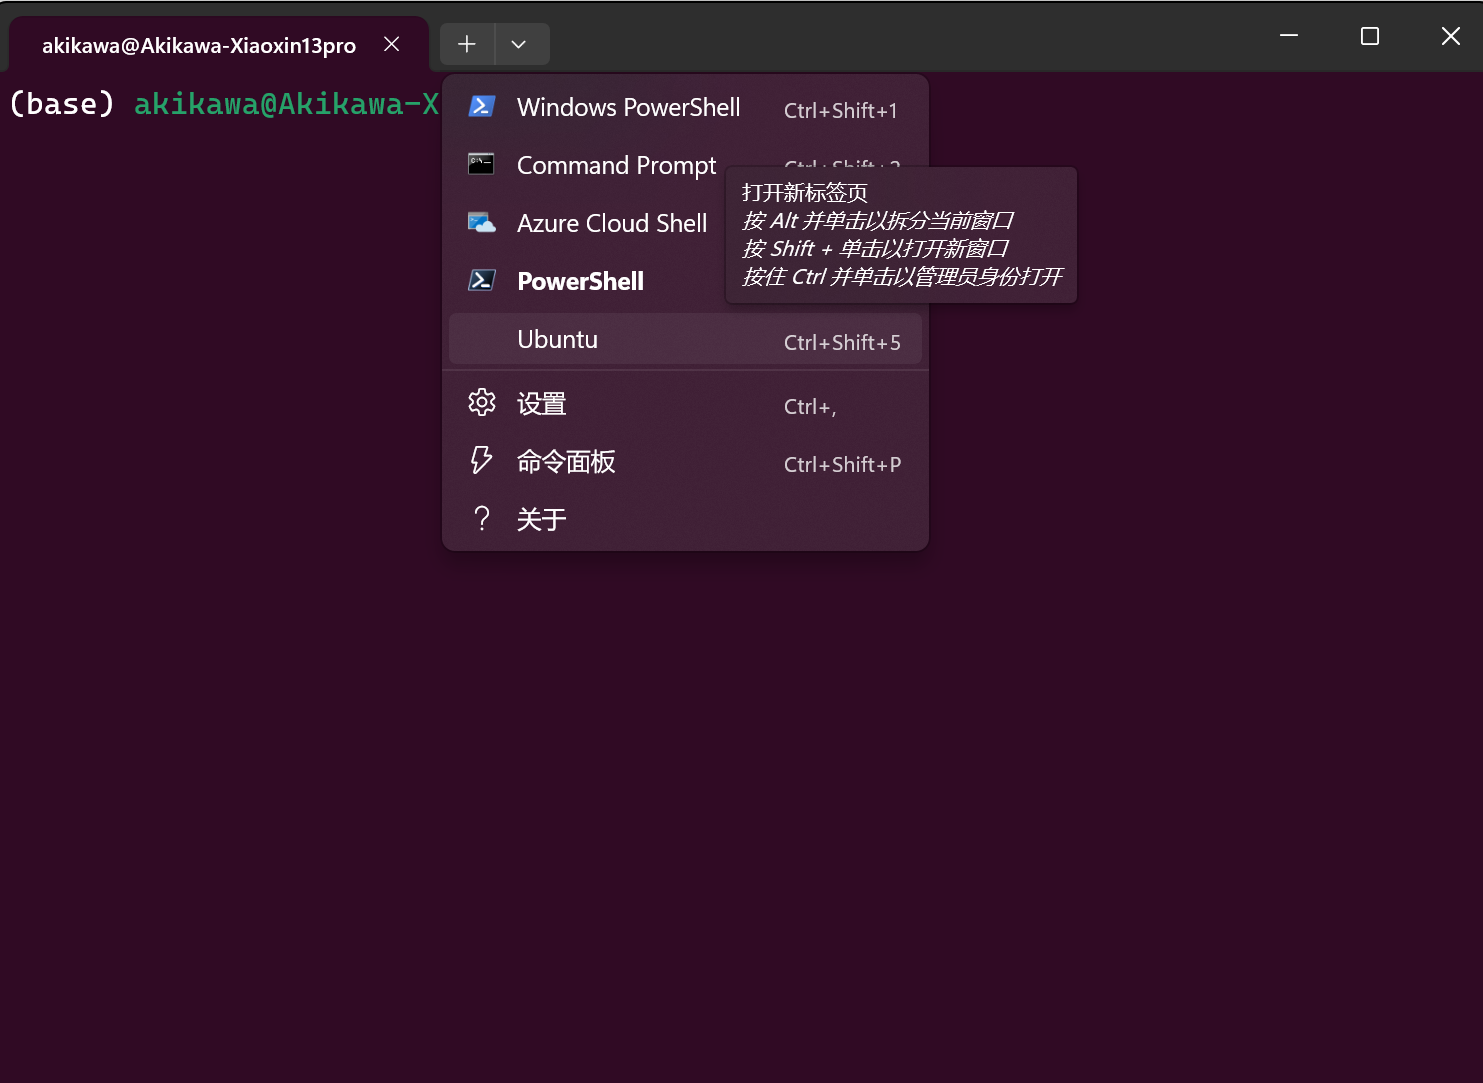
\includegraphics[width=13cm]{image/env/wsl-ubuntu.png}
    \caption{在终端中打开wsl}
    \label{ubuntu}
\end{figure}

\section{conda:环境管理系统}
Conda 是一个开源的包管理系统和环境管理系统,可在 Windows、macOS 和 Linux 上运行。 Conda 可快速安装、运行和更新包及其依赖项。 Conda 可以轻松地在计算机上创建、保存、加载和切换环境。 它是为 Python 程序而创造的,但它可以打包和分发任何语言的软件。

\subsection{conda安装}
conda分为anaconda和miniconda两种,前者包含一个基础的python环境,其中预装了常用的包;而后者较为精简,后续所有需要的东西可自行安装。这里展示miniconda的下载和安装过程,anaconda类似,只需要更改下载链接即可。

\subsubsection{conda下载}
以下是使用wget通过conda官网或者清华镜像源下载miniconda的代码,根据需要选择其一即可。
\begin{lstlisting}
    wget -c https://repo.continuum.io/miniconda/Miniconda3-latest-Linux-x86_64.sh
    wget -c https://mirrors.bfsu.edu.cn/anaconda/miniconda/Miniconda3-latest-Linux-x86_64.sh        #清华的镜像源latest的版本会一直更新到最新的版本
\end{lstlisting}

其中,-c表示断点续传。一般来说,如果没有VPN,清华镜像源下载速度较快,更为推荐。

\subsection{conda安装}
使用bash运行下载好的\lstinline{Miniconda3-latest-Linux-x86_64.sh}文件,如下:
\begin{lstlisting}
    bash Miniconda3-latest-Linux-x86_64.sh              #运行.sh 
\end{lstlisting}

安装过程中某一步会让你指定安装路径,如果有特殊需要可以改为你想安装到的路径(我将linux上安装的软件都放入了\lstinline{~/.app}中),否则全部选择yes即可。

\subsection{conda运行}
安装完成后,在终端中直接运行conda是无法启动的,你可以在\lstinline{~/.bashrc}中看见conda的路径,需要运行.bashrc文件进行初始化后方可进入conda环境,\lstinline{.bashrc}文件内容如下图:

\begin{figure}[ht]
    \centering
    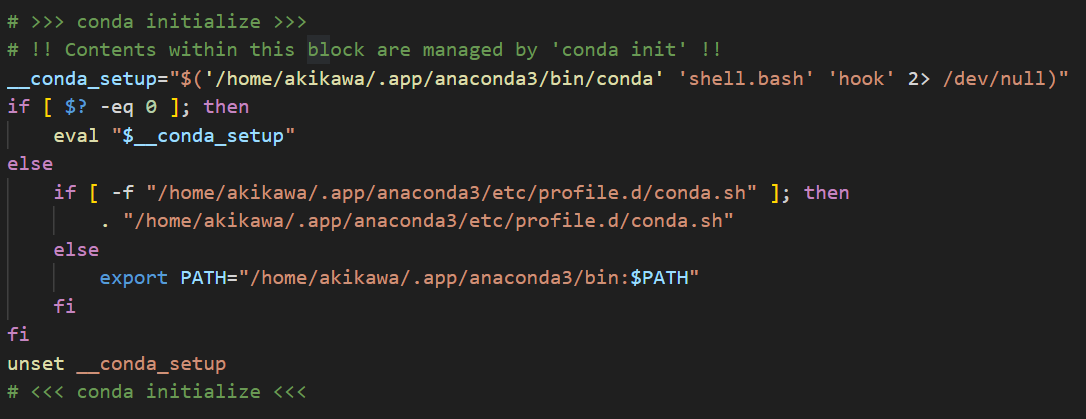
\includegraphics[width=13cm]{image/env/conda-initiate.png}
    \caption{.bashrc文件中的conda初始化部分}
\end{figure}

\subsection{环境}
环境是 conda 的重要概念,conda 可以创建各种环境,每个环境可以指定具体的 python 版本,可以在指定的环境下安装管理自己所需的包,并且环境之间相互隔离,互相不影响,类似命名空间的作用,对于不同需求场景下可以进行环境的自由切换,以下是与环境相关的一些简单命令,可在终端中打开Ubuntu后输入以下命令执行对应操作。
\begin{lstlisting}
    # 创建环境
    conda create -n forfun python=3.6
    # 列出所有环境
    conda env list
    # 删除环境
    conda env remove -n forfun
    # 激活环境
    source activate forfun
    # 退出环境
    source deactivate
\end{lstlisting}

在某个环境下,可以通过下述命令管理包
\begin{lstlisting}
    # 检索可以下载的包
    conda search numpy
    # 下载包
    conda install numpy  
    # 移除包
    conda remove numpy  
    # 列出所有安装包
    conda list
\end{lstlisting}


\section{VSCode:轻量化集成代码编辑器}
VSCode 全称 Visual Studio Code,是微软出的一款轻量代码编辑器,免费、开源而且功能强大。它支持几乎所有主流的程序语言的语法高亮、智能代码补全、自定义热键、括号匹配、代码片段、代码对比 Diff、GIT 等特性,支持插件扩展,并针对网页开发和云端应用开发做了优化。软件跨平台支持 Win、Mac 以及 Linux。

\subsection{VSCode安装及中文环境配置}
打开 \href{https://code.visualstudio.com/}{VSCode官网},点击下载链接即可s下载安装。下载简体中文插件后即可将语言切换为中文。此后,如需配置对应的环境,如Python、R、Latex环境,只需下载主程序后\footnote{因为本质上VSCode只是一个壳,和记事本类似,程序的运行是在对应终端中进行的}在VSCode中安装对应的包即可。

\begin{remark}
    VSCode除了各类代码,还可以方便地打开xml、csv、xlsx、docx、tif、html、svg等常见文件,只要安装对应的插件即可;也可以直接对文本文件进行编辑,因而VSCode为没有图形化界面的WSL增添了许多便利。
\end{remark}

\subsection{VSCode连接WSL、SSH}
安装好WSL后,在VSCode左侧侧边栏的Remote Explorer分区,你可以在上方选择WSL Target直接连接到子系统,方便完成文本编辑,文件预览,文件传输等功能(可将Windows上文件直接拖动到VSCode的资源管理器中完成上传,将WSL上文件通过右键点击完成下载)等功能



\subsection{在VSCode上通过SSH连接远程Linux服务器}
\subsubsection{在VSCode中配置SSH}
\begin{quotation}
    本部分参考CSDN上部分文章\cite{ssh},结合我们自身配置过程书写而成。
\end{quotation}
在win10中安装open-SSH客户端,可使用“应用与程序”或“windows power shell”,如图\ref{win-ssh}。
\begin{figure}[ht]
    \centering
    \begin{minipage}[c]{0.45\textwidth}
        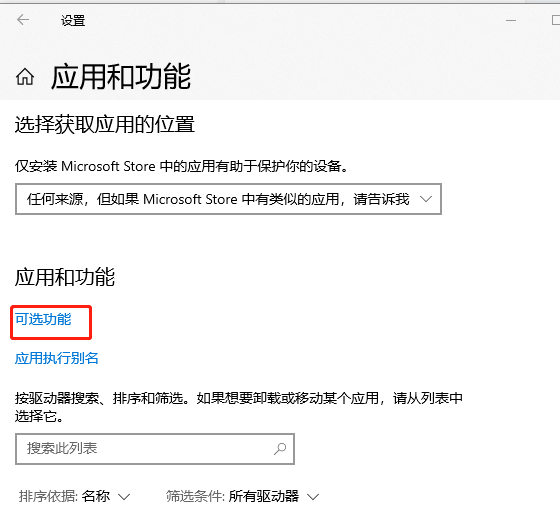
\includegraphics[width=\textwidth]{image/env/win-ssh.png}
    \end{minipage}
    \begin{minipage}[c]{0.45\textwidth}
        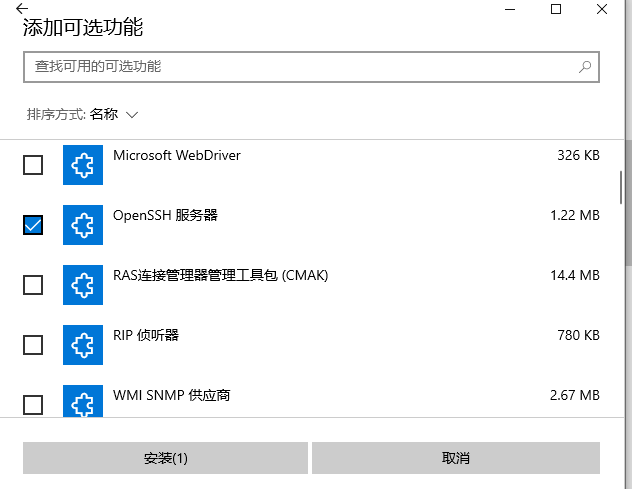
\includegraphics[width=\textwidth]{image/env/win-ssh2.png}
    \end{minipage}

    \caption{Win10中安装OpenSSH}
    \label{win-ssh}
\end{figure}

在vs-code的extension中搜索remote-ssh并安装
\begin{figure}[ht]
    \centering
    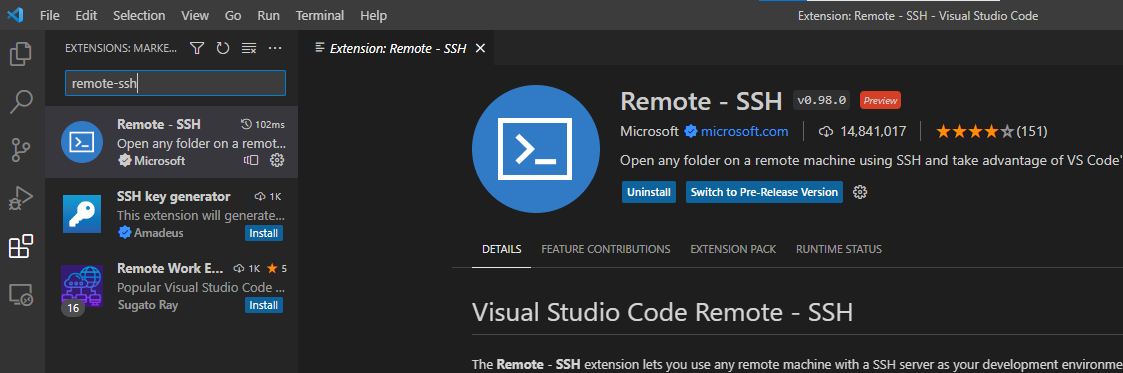
\includegraphics[width=13cm]{image/env/vsc-plugin.png}
\end{figure}

配置.config文件
\begin{figure}[ht]
    \centering
    \begin{minipage}[c]{0.65\textwidth}
        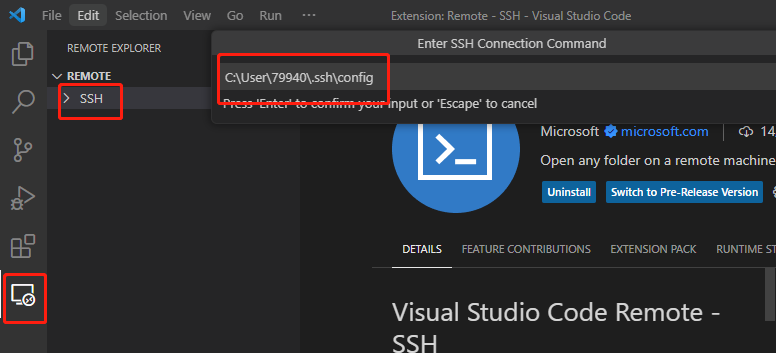
\includegraphics[width=\textwidth]{image/env/vs-ssh-config.png}
    \end{minipage}
    \begin{minipage}[c]{0.3\textwidth}
        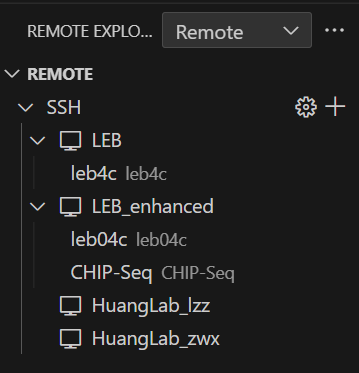
\includegraphics[width=\textwidth]{image/env/vs-remote.png}
    \end{minipage}
    \caption{VSCode中配置SSH远程连接}
    \label{vs-ssh}
\end{figure}

\begin{lstlisting}
    Host LEB
    HostName 117.78.18.116
    User leb4c

    Host LEB_enhanced
    HostName 114.115.164.221
    User leb04c
\end{lstlisting}

其中,Host、HostName和User分别表示你希望显示在本地的服务器名称,服务器SSH地址和你在服务器上登录的用户名。保存后可直接点击列表内的服务器登录,如图\ref{vs-ssh}右所示。

右键添加扩展设置。
\begin{figure}[ht]
    \centering
    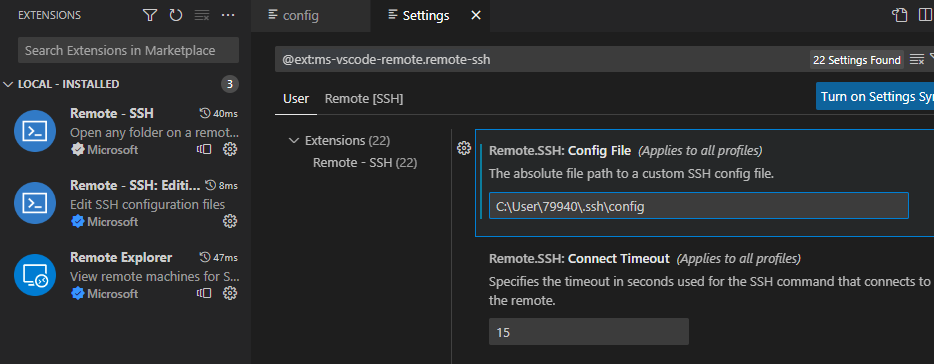
\includegraphics[width=13cm]{image/env/vs-ssh-plugin-set.png}
\end{figure}

勾选首选项中显示登录窗口,以输入密码
\begin{figure}[ht]
    \centering
    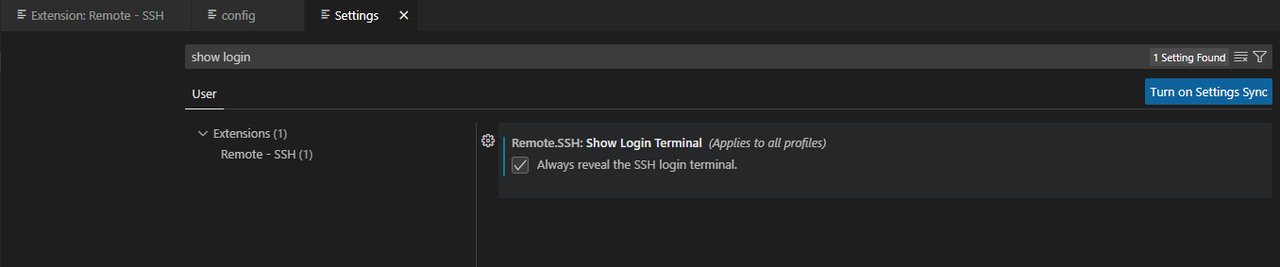
\includegraphics[width=13cm]{image/env/vs-remote-show-login.png}
\end{figure}

在VSCode中登录并在提示后输入密码,如图\ref{login}。

\begin{figure}[ht]
    \centering
    \begin{minipage}[c]{0.9\textwidth}
        \centering
        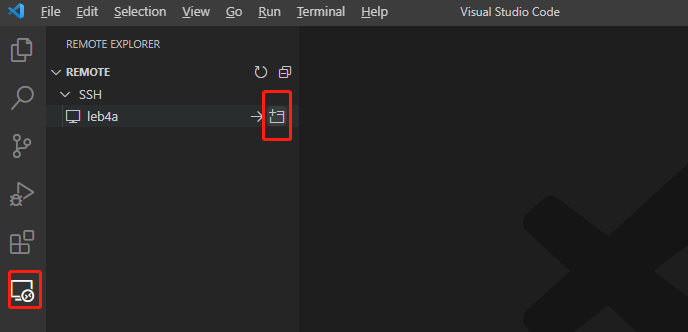
\includegraphics[width=13cm]{image/env/ssh-login.png}
    \end{minipage}

    \begin{minipage}[c]{0.9\textwidth}
        \centering
        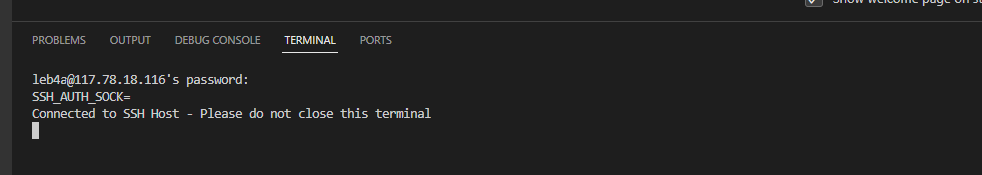
\includegraphics[width=13cm]{image/env/pswd.png}
    \end{minipage}
    \caption{VSCode中登录}
    \label{login}
\end{figure}

可以通过VSCode清晰展示各个文件、路径,可在展示termial的同时修改文件内容,如图\ref{vsc-page}。
\begin{figure}[ht]
    \centering
    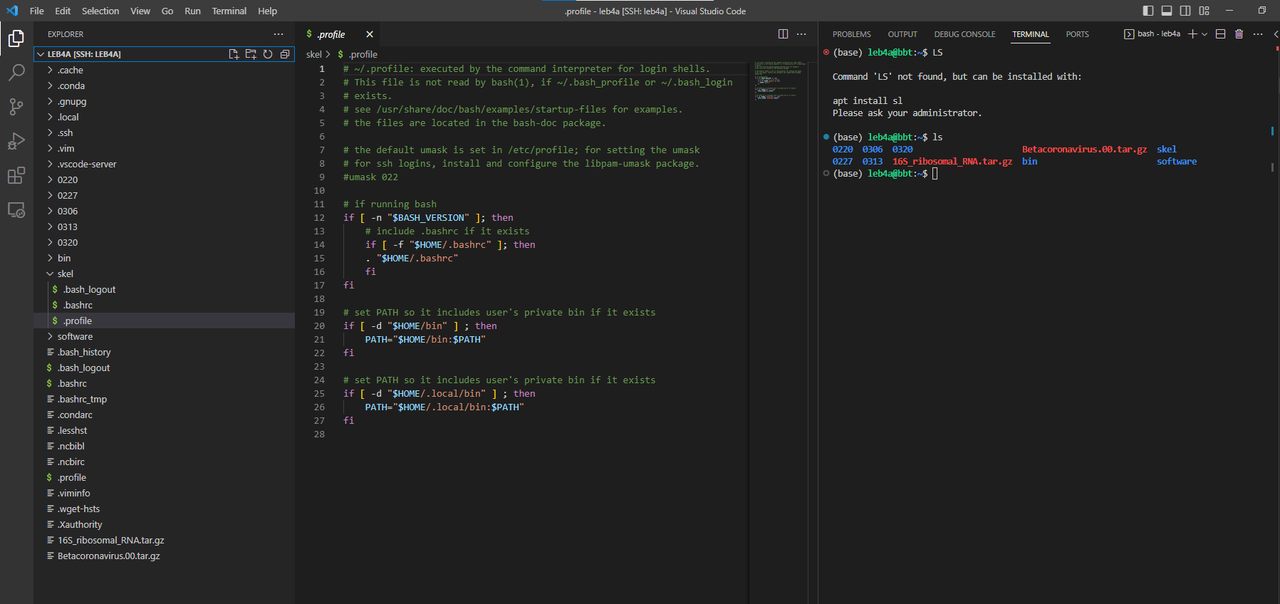
\includegraphics[width=13.5cm]{image/env/vs-remote-show.png}
    \caption{VSCode连接服务器后的页面}
    \label{vsc-page}
\end{figure}

\subsubsection{配置SSH免密码登录}
\begin{quotation}
    \textit{本部分参考CSDN上部分文章\cite{ssh-nopswd},结合我们自身配置过程书写而成。该部分主要针对Windows用户,MacOS用户配置过程类似,不过在获取密钥和复制密钥部分有所不同,需要留心。}
\end{quotation}

首先,使用\lstinline{win+R}进入cmd,在cmd中输入\lstinline{ssh-keygen -t rsa}获取密钥,如图\ref{vs-ssh-miyao},文件中生活蹭了公钥和私钥。
\begin{figure}[ht]
    \centering
    \begin{minipage}[c]{0.9\textwidth}
        \centering
        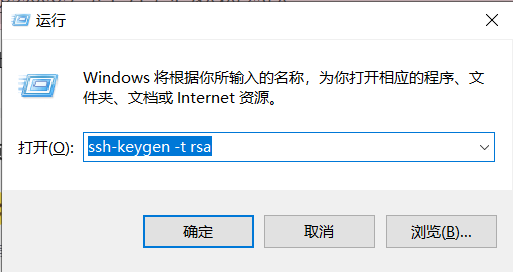
\includegraphics[width=10cm]{image/env/ssh-miyao.png}
    \end{minipage}

    \begin{minipage}[c]{0.9\textwidth}
        \centering
        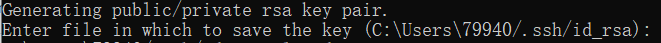
\includegraphics[width=10cm]{image/env/ssh-miyao2.png}
    \end{minipage}

    \begin{minipage}[c]{0.9\textwidth}
        \centering
        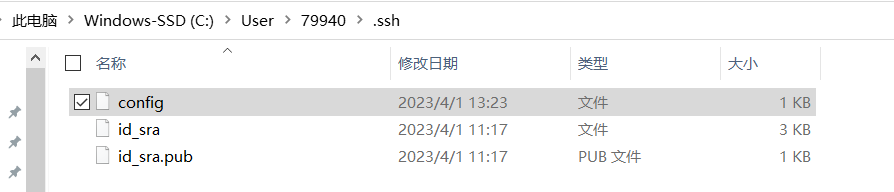
\includegraphics[width=10cm]{image/env/ssh-miyao3.png}
    \end{minipage}

    \caption{在CMD中生成密钥}
    \label{vs-ssh-miyao}
\end{figure}

然后,在配置文件中添加密钥地址,注意为不含.pub后缀的文件
\begin{lstlisting}
# Read more about SSH config files: https://linux.die.net/man/5/ssh_config
Host leb4a
HostName 117.78.18.116
# 服务器地址
User leb4a
# 登录服务器时的用户名
PreferredAuthentications publickey
IdentityFile "C:\Users\79940\.ssh\id_rsa"
# 本地密钥文件地址
\end{lstlisting}

在服务器下.shh文件夹中,使用touch新建authorized\_keys许可文件,将公钥.pub文件中的内容复制到authorized\_keys中,如图\ref{.pub},即可完成不输入密码登录。
\begin{figure}[ht]
    \centering
    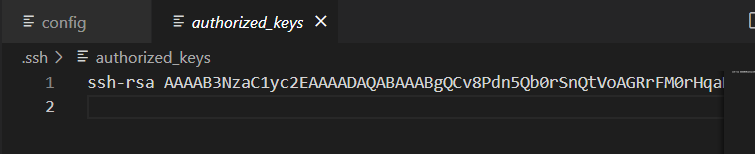
\includegraphics[width=13cm]{image/env/ssh-miyao-fuwuqi.png}
    \caption{将.pub文件中内容复制到服务器}
    \label{.pub}
\end{figure}


\section{实例:VSCode中使用JupyterNotebook运行R}
Conda除了可以配置python环境,也可以用于配置和管理R环境,以此将不同项目所用的R环境隔开,减少package加载时间,同时防止package冲突。这里,我们利用conda在WSL中配置R的JupyterNotebook环境并在VSCode中编辑与运行。

\subsection{用conda配置R环境}
\begin{lstlisting}
    conda create -n r_env r-base=4.3.0 r-essentials
    # -n 指定r环境名称,此处为"r_env"
    # r-base=xx, 设置r版本
    # r-essentials, 基础Rpackages,选装
    conda activate r_env
\end{lstlisting}

\subsection{安装package}
如果用conda安装r包,需要切换对应的到r环境下,如(r\_env),且包名前需要加"r-",如\lstinline{conda install r-package\_name}

但更推荐的是使用r的包管理应用安装包,如BiocManager。

在终端中切换到r\_env,并启动R,然后使用BiocManager安装需要的包。需要注意的是此步需要在终端内完成,不能在JupyterNotebook中完成,否则无法连接网络。

\begin{lstlisting}
    # 启动R环境
    R

    # 以下已经进入R环境
    # 如果没有BiocManager就安装BiocManager
    if (!requireNamespace("BiocManager", quietly = TRUE))
    install.packages("BiocManager")

    # 用BiocManager安装对应包
    BiocManager::install("DESeq2")
    BiocManager::install("readxl")
    BiocManager::install("EnhancedVolcano")
\end{lstlisting}

\subsection{在vsCode中使用JupyterNotebook运行R程序}
利用conda下载JupyterNotebook for R的核心插件irkernel

\begin{lstlisting}
    conda install -c r r-irkernel
\end{lstlisting}

然后就可以使用网页端JupyterNotebook了!命令如下:
\begin{lstlisting}
    conda activate r_env
    jupyter notebook
\end{lstlisting}

或者也可以在VSCode中选择kernel(安装irkernel后需要先重启VSCode才能看到内核)

\begin{figure}[ht]
    \centering
    \begin{minipage}[c]{0.9\textwidth}
        \centering
        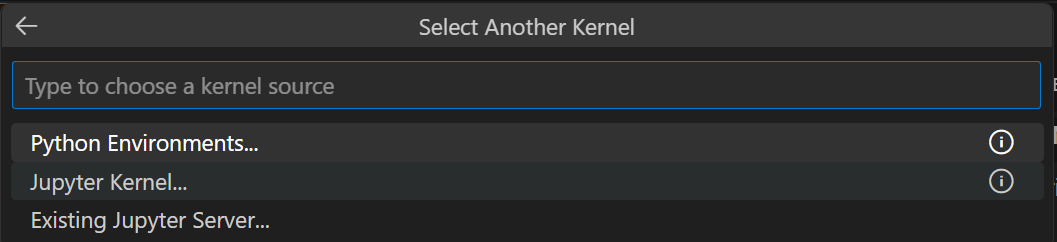
\includegraphics[width=13cm]{image/env/jupyter-list.png}
    \end{minipage}

    \begin{minipage}[c]{0.9\textwidth}
        \centering
        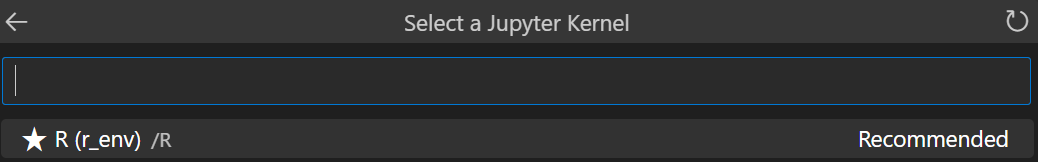
\includegraphics[width=13cm]{image/env/jupyter-r-list.png}
    \end{minipage}
    \caption{在VSCode中选择JupyterNotebook的内核}
\end{figure}

这样,就可以在vscode中愉快地使用R了!